\newpage
\subsection{Connected Components}
\begin{definition}[]{Connected Component}
    A \textbf{connected component} of a graph $G = (V, E)$ is a maximal subset of vertices $C \subseteq V$ such that:
    \begin{itemize}
        \item For every pair of vertices $u, v \in C$, there exists a path connecting $u$ and $v$.
        \item Adding any vertex $w \notin C$ to $C$ would violate the connectedness condition.
    \end{itemize}
\end{definition}

\begin{remarks}[]{Key Points About Connected Components}
    \begin{itemize}
        \item \textbf{Undirected Graphs:} A connected component is a subgraph where any two vertices are connected by a path, and which is connected to no additional vertices in the graph.
        \item \textbf{Directed Graphs:} There are two types of connected components:
              \begin{itemize}
                  \item \textbf{Strongly Connected Component:} A maximal subset of vertices where every vertex is reachable from every other vertex (considering edge direction).
                  \item \textbf{Weakly Connected Component:} A maximal subset of vertices where connectivity is considered by ignoring edge directions.
              \end{itemize}
    \end{itemize}
\end{remarks}

\begin{example}[]{Connected Components in a Graph}
    \begin{center}
        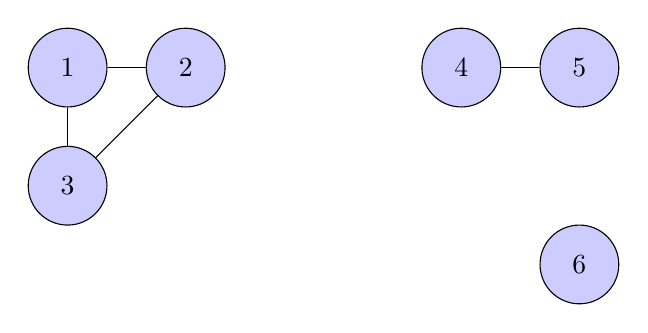
\begin{tikzpicture}[node distance=1.5cm, main/.style={circle, draw, fill=blue!20, minimum size=10mm, inner sep=0pt}]
            % Connected component 1
            \node[main] (1) {1};
            \node[main] (2) [right of=1] {2};
            \node[main] (3) [below of=1] {3};
            \draw (1) -- (2);
            \draw (1) -- (3);
            \draw (2) -- (3);

            % Connected component 2
            \node[main] (4) [right of=2, xshift=2cm] {4};
            \node[main] (5) [right of=4] {5};
            \draw (4) -- (5);

            % Isolated vertex (another component)
            \node[main] (6) [below of=5, yshift=-1cm] {6};
        \end{tikzpicture}
    \end{center}
\end{example}

\begin{remarks}[]{Understanding the Example}
    \begin{itemize}
        \item In the given undirected graph:
              \begin{itemize}
                  \item \textbf{Component 1:} $\{1, 2, 3\}$ (fully connected subgraph).
                  \item \textbf{Component 2:} $\{4, 5\}$ (connected by a single edge).
                  \item \textbf{Component 3:} $\{6\}$ (an isolated vertex).
              \end{itemize}
        \item These subsets are disjoint and collectively partition the graph's vertex set $V$.
    \end{itemize}
\end{remarks}
